\documentclass{article}
\usepackage[utf8]{inputenc}
\usepackage[document]{ragged2e}
\usepackage{algpseudocode}
\usepackage[]{algorithmicx}
\usepackage{amsmath}
\usepackage{amsthm}
\usepackage{amssymb}
\usepackage[]{listings}
\usepackage{graphicx}
\usepackage{hyperref}
\usepackage{flafter}
\usepackage{subfig}
\usepackage{dsfont}
\usepackage[T1]{fontenc}
\graphicspath{ {images/} }

\begin{document}

\begin{titlepage}
	\centering
	%
\includegraphics[width=0.15\textwidth]{IIIT-B_logo.jpg}\par\vspace{1cm}
	{\scshape\LARGE International Institute of Information Technology, Bangalore \par}
	\vspace{1cm}
	{\scshape\Large Project Strategy Document\par}
	{\Large  DS 707 Data Analytics\par}
	\vspace{1.5cm}
	{\huge\bfseries Clustering and Association \par}
	\vspace{2cm}
	{\Large\itshape Akanksha Dwivedi - MT2016006\par}
	{\Large\itshape Hitesha Mukherjee - MS2016007\par}
	{\Large\itshape Nayna Jain - MS2017003\par}
	{\Large\itshape Tarini Chandrashekhar - MT2016144\par}
	\vfill
	Instructors : \par
	Prof. Ramanathan Chandrashekhar
	\par
	Prof. Uttam Kumar

	\vfill
% Bottom of the page
	{\large \today\par}
\end{titlepage}

\newpage

\section{Introduction}
As with stock market, cryptocurrency is growing investment area for the daily traders and investors. Cryptocurrency is very new and still stabilizing. Because of which it is very volatile in nature and might get affected by different factors. In such an environment it is very difficult to predict the price movement of cryptocurrencies.

Since the trend and investment point of view is similar to stock market, the established techniques used in stock market prediction are considered
or cryptocurrency.

[1][2] refers to the papers which shows how clustering is used in the process of stock price prediction.

We have applied similar techniques from [1] for the cryptocurrency forecasting.
[1] discusses three steps for forecasting which are:
\begin{itemize}
	\item Normalizing the data
	\item K-means clustering of the normalized data to identify the outliers
	\item ARIMA for forecasting on clustered data.
\end{itemize}

Thus, we see how clustering is applied to remove the outliers from the clusters.

\section{Clustering Techniques}
\subsubsection{K-Means Clustering}

It is a centroid based partitioning technique that uses the centroid of a cluster, Ci to represent the cluster. Conceptually, the centroid of a cluster is its center point. This algorithm requires to specify the number of clusters (k) beforehand. This method is not guaranteed to converge to the global optimum and often terminates to a local optimum.

We have applied this algorithm on Open/High attributes of the daily prices. And with some experimentation, of taking no of clusters values from 3, 4, 5, we found that between 4 and 5 here is not much difference. And so we decided to take the k value as 4. We attempt to identify the outliers based on these attributes.

\begin{figure}[ht]
	\centering
	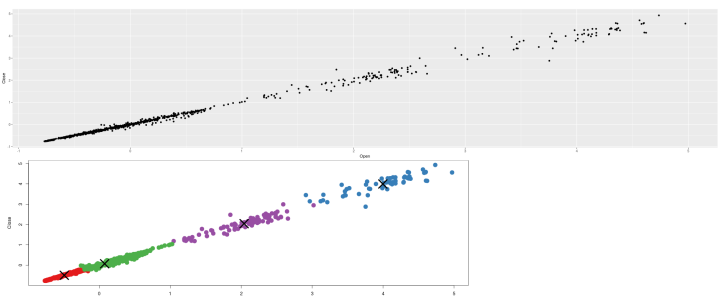
\includegraphics[scale=0.25]{images/KMeansClustering}
	\caption{Before and After K Means Clustering}
	\label{fig:kmeansclustering}
\end{figure}

\section{Time Series}

\subsection{Introduction}

Time Series data is the collection of observations which are collected over a period of time, generally over a fixed intervals. The data can be univariate or multi-variable based on number of attributes we want to apply timeseries on. Time series data analysis is applied for the purpose of:

\begin{itemize}
	\item Understanding what happened in the past (Trend).
	\item Predicting/Forecasting the future.
\end{itemize}

\subsection{Stationary Series}
One of the basic requirement for time series modeling is to first check whether the data is stationary or non-stationary. The data is said to be stationary if it satisfies the following  property:

\begin{itemize}
	\item The mean of the series should not be a function of time but should be a constant.
	\item The variance of the series should not be a function of time.
	\item The co-variance of the ith term and (i + m)th term should not be a function of time.
\end{itemize}

So, for the time series modeling, if the data is not stationary, it has to be first converted into stationary data.
To verify whether data is stationary or not, we can use Dickey Fuller Test of Stationarity.
For the Dickey-Fuller Test, the p value has to be less than 0.05 or 5.
If it satisfies the above condition, it is considered as stationary series, else it is a non-stationary series.
To convert non-stationary into stationary, differencing should be applied before proceeding.


\subsection{Time Series Components}
There are four components of the Time Series:

\begin{itemize}
	\item Trend Component:
	Movement of data over a period of time like whether increasing, decreasing or remaining unchanged is defined as Trend.
	\item Seasonal Component:
	Fluctuations observed during specific seasons or chunks of time. Eg.. during 4th quarter of very year, stocks tends to show better.
	\item Cycle Component:
	Some type of data tends to repeat itself over a longer period of time, thereby exhibiting some cycles. It can be combination of trend and seasonal data.
	\item Irregular Component:
	Randomness or noise in the data.
\end{itemize}	

The time series modelling can be represented as additive or multiplicative model.
Additive Model:\linebreak
Y(t) = T(t) + S(t) + C(t) + R(t)\linebreak
\linebreak
Multiplicative Model:\linebreak
Y(t) = T(t) * S(t) * C(t) * R(t)\linebreak
\linebreak
where,\linebreak
T - Trend\linebreak
S - Seasonal\linebreak
C - Cycle\linebreak
R - Random\linebreak

\subsection{Identify p, d and q for ARIMA models}
	
	The two key concepts which helps in identifying the p and q values used in AR(p) and MA(q), are ACF and PACF
	
	\subsubsection{Autocorrelation Function(ACF)}
	It is a correlation function which rather than showing correlation between two different variables, the correlation is between different values of same variable i.e Xi and Xi+k.\linebreak
	ACF is used to identify the q value for MA component of ARIMA. To calculate the MA term of the model, the lag at which the ACF cuts is considered. It displays the sharp cut-off at the negative correlation.

	
\subsubsection{Partial Autocorrelation Function(PACF)}

It is also a correlation function, but it gives the partial correlation of time series with its own lagged values, controlling for the values of the time series at all shorter lags. It contrasts with the autocorrelation function, which does not control the other lags.\linebreak
PACF is used to identify the p value for the AR component of ARIMA.
The lag at which the PACF cuts off is the indicated number of AR terms. It displays a sharp cutoff at the positive autocorrelation.

\subsection{Finalizing values for p, d and q}

\begin{itemize}
	\item p - This is calculated by finding the lag k via PACF function
	\item d - This is the differencing order used while making the data stationary
	\item q - This is calculated by finding the lag k via ACF function.
\end{itemize}

\subsection{Generating ARIMA model}

After identifying the values of p, d and q, we can create the ARIMA model.
The ARIMA model can then be used to forecast or predict the future values.\linebreak

ARIMA model can be validated by examining ACF and PACF for residual models.
After fitting the correct model, it can then be used to do forecast and prediction.\linebreak
We can also verify the forecast and prediction, by reserving a portion of our dataset and applying the prediction on top of it, thereby comparing the forecasted and actual
observed values.



\section{Applying ARIMA on bitcoin\_price dataset}

Dataset used: bitcoin\_price.csv  \linebreak
Attribute used for modelling - Close Price  \linebreak
ARIMA model - univariate analysis as trading prices are often analyzed based on how they had been behaving over the period of time. \linebreak
Data has been cleaned before applying ARIMA model. \linebreak

\subsection{Exploring Raw Data}

Plot for visualizing the raw data as obtained is shown in Figure 2.


\begin{figure}[ht]
	\centering
	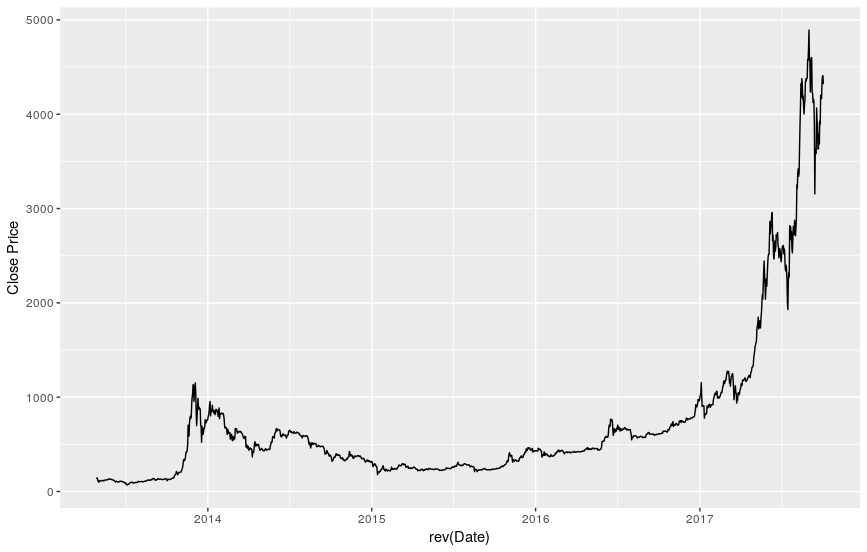
\includegraphics[scale=0.30]{images/ts_images/RawClosePricePlot.png}
	\caption{Original Raw Close Price Data}
	\label{fig:Original Raw Close Price Data}
\end{figure}

With the K-Means clustering it was identified, that there existed some outliers.
So, with tsclean function of R, data has been cleaned for outliers to avoid any skewing.\linebreak Figure 3 shows clean data.

\begin{figure}[ht]
	\centering
	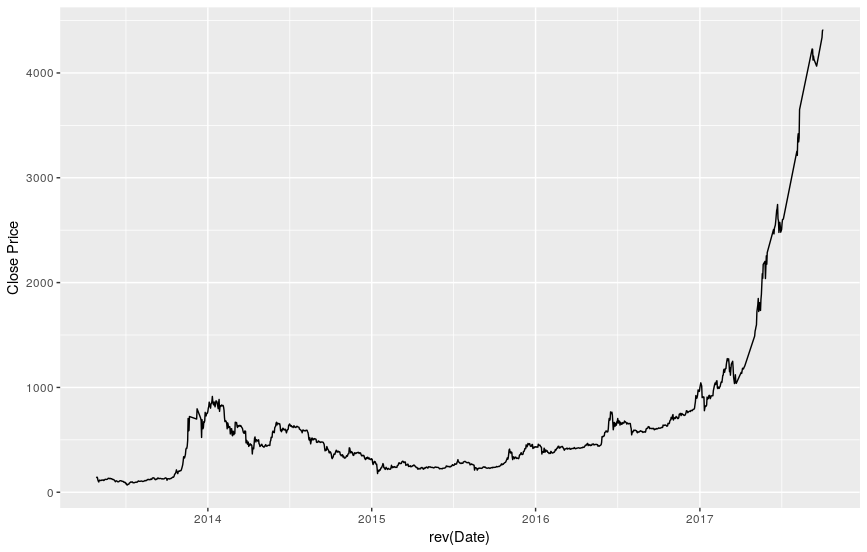
\includegraphics[scale=0.30]{images/ts_images/CleanedClosePricePlot.png}
	\caption{Cleaned Close Price Data}
	\label{fig:Cleaned Close Price Data}
\end{figure}


As part of exploration, we also calculated the moving average data. However, this moving average was to smoothen the data rather than actual modelling.
Further analysis is done on dataset with this moving average value.\linebreak Figure 4. shows the smoothened data.

\begin{figure}[ht]
	\centering
	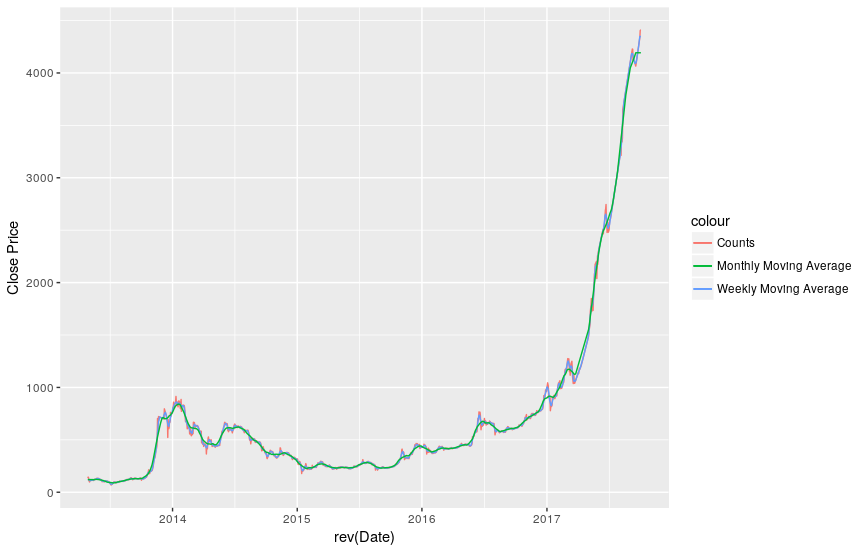
\includegraphics[scale=0.30]{images/ts_images/MovingWeeklyAverage.png}
	\caption{Moving Average Data}
	\label{fig:Moving Average Data}
\end{figure}

\subsection{Trend Components}
Figure 5 shows the trend, seasonal and residual components for the dataset

\begin{figure}[ht]
	\centering
	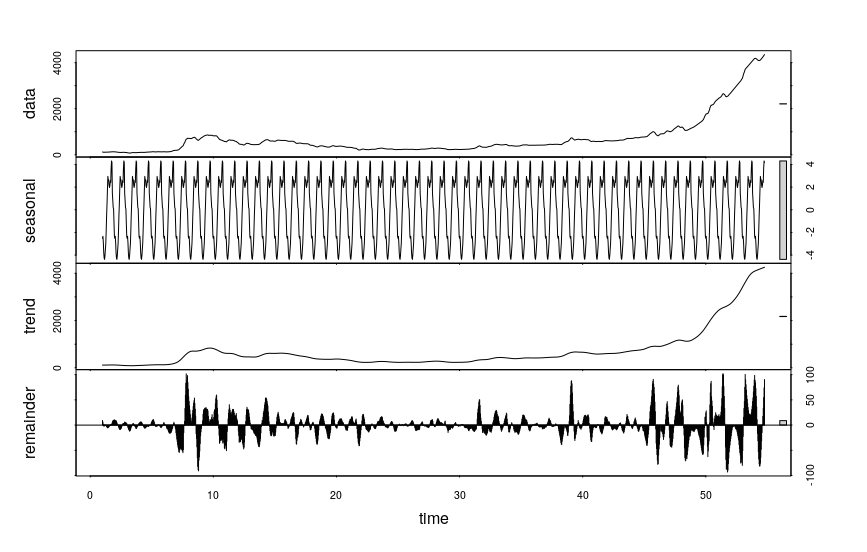
\includegraphics[scale=0.25]{images/ts_images/TimeSeriesComponents.png}
	\caption{Time Series Components}
	\label{fig:Time Series Components}
\end{figure}

Since there did exist some seasonal component, we subtracted it as shown in Figure 6.


\begin{figure}[ht]
	\centering
	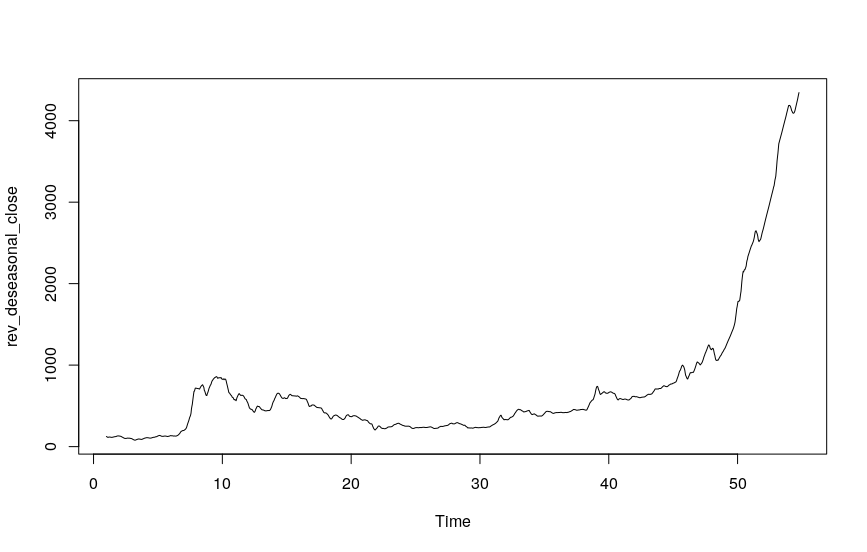
\includegraphics[scale=0.25]{images/ts_images/SubtractingSeasonal.png}
	\caption{Subtracting Seasonal Components}
	\label{fig:Subtracting Seasonal Components}
\end{figure}

Further analysis is done on data after subtracting seasonal components.

\subsection{Stationary Series}

Next step identifies if the data is stationary or not, by applying Dickey Fuller Test and verifying with Plot.
\subsubsection{Differencing 0}
Without any differencing, the result of Dickery Fuller Test, showed following value

p-value = 0.99 \linebreak
alternative hypothesis: stationary \linebreak
Since p-value > 0.05, it applied that there is a need of differencing. It can also be seen from Figure (Cleaned Close Price Data)
This is applied without differencing so is same as Figure 3.

\subsubsection{Differencing 1}
Differencing value as 1, the result of Dickery Fuller Test, showed following value

p-value = 0.01 \linebreak
alternative hypothesis: stationary \linebreak
Since p-value < 0.05, it applied that there data is now stationary as also seen from Figure 7 for differenced Close Price Data.

\begin{figure}[ht]
	\centering
	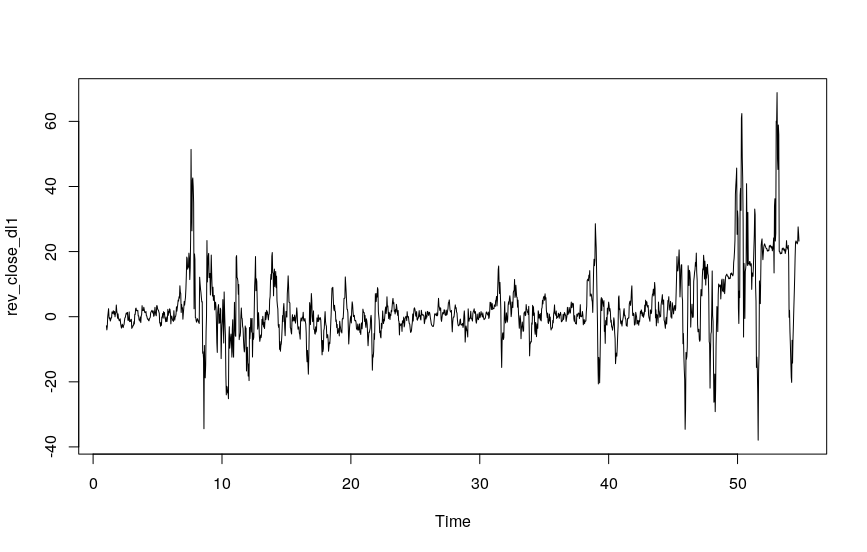
\includegraphics[scale=0.25]{images/ts_images/CloseWithDifferencing1.png}
	\caption{Close Price after 1 order differencing}
	\label{fig:Close Price after 1 order differencing}
\end{figure}

\subsubsection{Differencing 2}
Differencing value as 2, the result of Dickery Fuller Test, showed following value

p-value = 0.01 \linebreak
alternative hypothesis: stationary \linebreak
Since p-value < 0.05, it applied that there data is now stationary as also seen from Figure 8 for differenced Close Price Data.

\begin{figure}[ht]
	\centering
	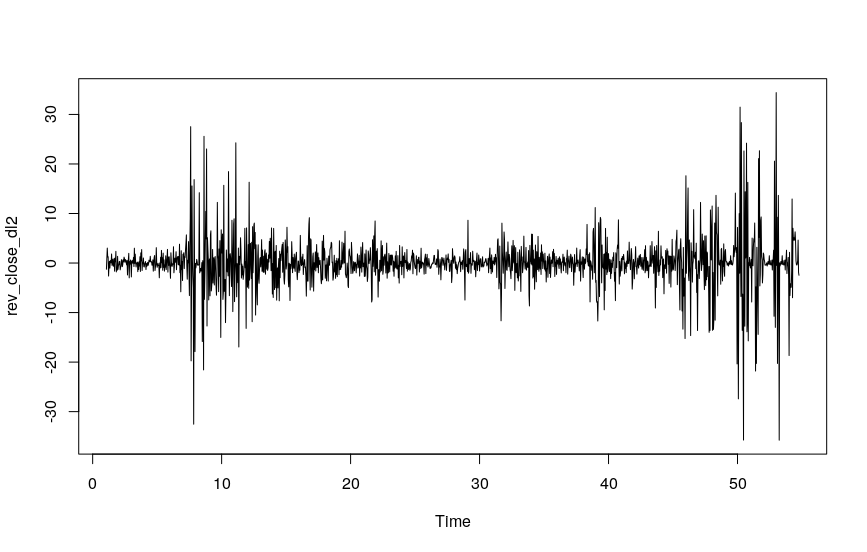
\includegraphics[scale=0.25]{images/ts_images/CloseWithDifferencing2.png}
	\caption{Close Price after 2 order differencing}
	\label{fig:Close Price after 2 order differencing}
\end{figure}


Since both with d = 1 and d = 2, we get p < 0.01, we can choose any of these for further analysis. However, if we see the plots we see that the graph with d = 2 is more around 0 value rather than d = 1. And so we 
decide to take d = 2 for further analysis.

\subsection{Identify p, d and q for ARIMA models}

\subsubsection{ACF and PACF for Differencing 0}

Figure 9 and 10 shows ACF and PACF plots for data without any differencing.

\begin{figure}[ht]
	\centering
	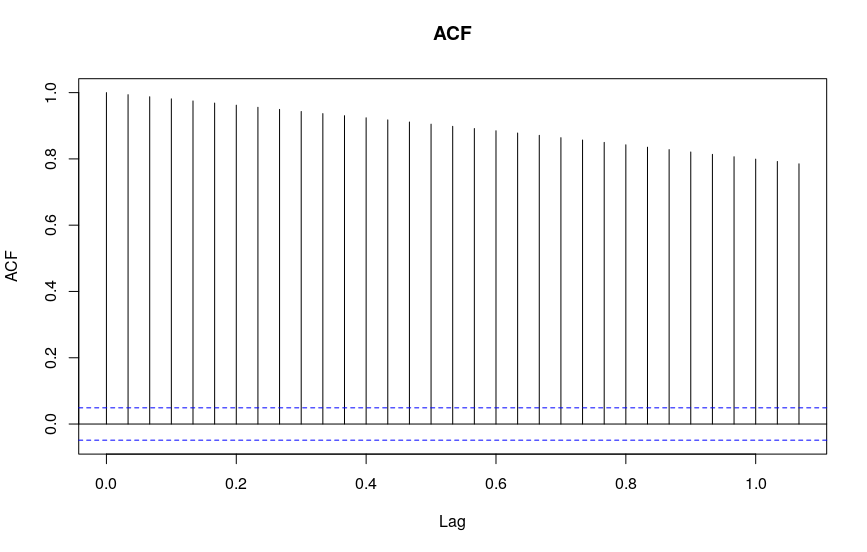
\includegraphics[scale=0.25]{images/ts_images/ACFWith0Differencing.png}
	\caption{ACF with 0 order differencing}
	\label{fig: ACF with 0 order differencing}
\end{figure}

\begin{figure}[ht]
	\centering
	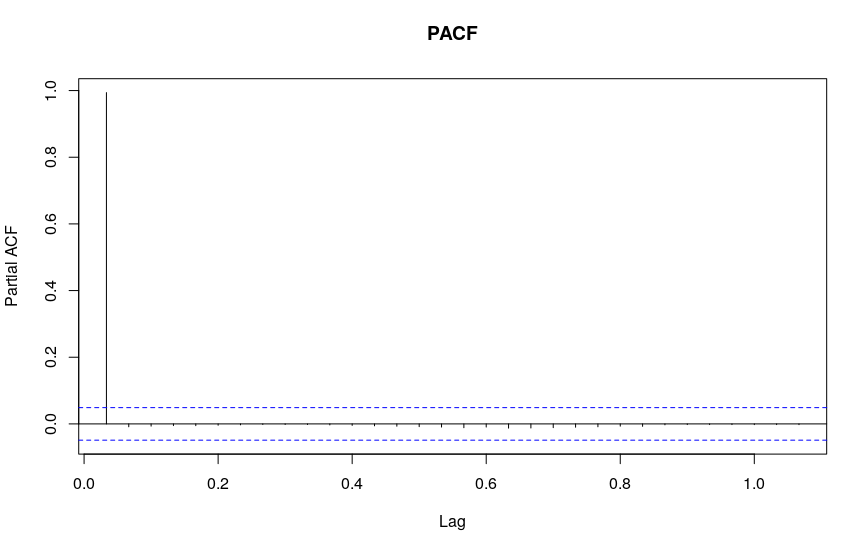
\includegraphics[scale=0.25]{images/ts_images/PACFWith0Differencing.png}
	\caption{PACF with 0 order differencing}
	\label{fig: PACF with 0 order differencing}
\end{figure}

\subsubsection{ACF and PACF for Differencing 1}

Figure 11 and 12 shows ACF and PACF plots for data with differencing order 1.

\begin{figure}[ht]
	\centering
	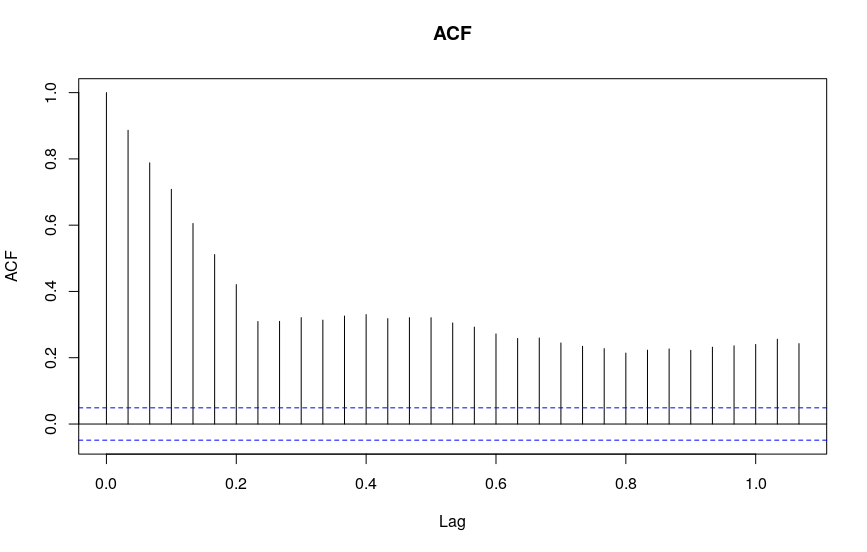
\includegraphics[scale=0.25]{images/ts_images/ACFWith1Differencing.png}
	\caption{ACF with 1 order differencing}
	\label{fig: ACF with 1 order differencing}
\end{figure}

\begin{figure}[ht]
	\centering
	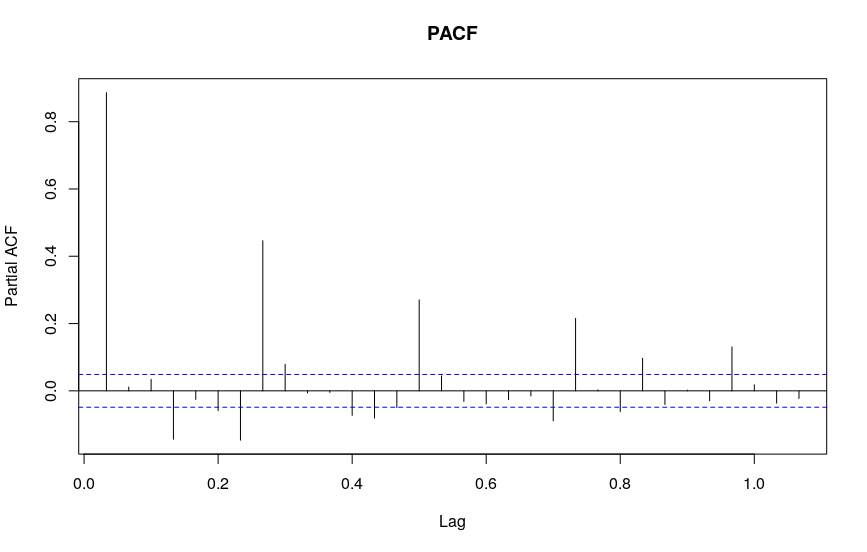
\includegraphics[scale=0.25]{images/ts_images/PACFWith1Differencing.png}
	\caption{PACF with 1 order differencing}
	\label{fig: PACF with 1 order differencing}
\end{figure}

\subsubsection{ACF and PACF for Differencing 2}

Figure 13 and Figure 14 shows ACF and PACF for data with differencing order 2.

\begin{figure}[ht]
	\centering
	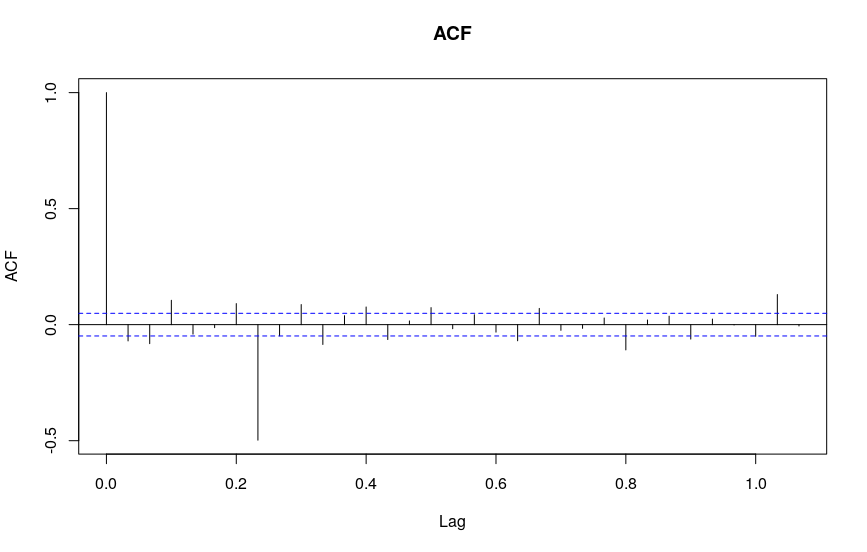
\includegraphics[scale=0.25]{images/ts_images/ACFWith2Differencing.png}
	\caption{ACF with 2 order differencing}
	\label{fig: ACF with 2 order differencing}
\end{figure}

\begin{figure}[ht]
	\centering
	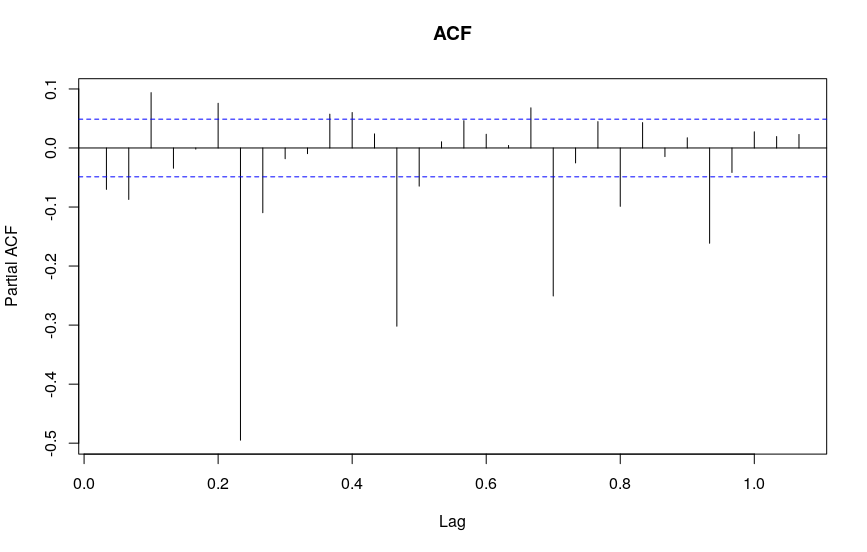
\includegraphics[scale=0.25]{images/ts_images/PACFWith2Differencing.png}
	\caption{PACF with 2 order differencing}
	\label{fig: PACF with 2 order differencing}
\end{figure}

We can see ACF and PACF plots for differencing order 1, 2, and 3 as above. And we see that ACF plot shows the lags in the graph with d = 2.
So, this again matches with our previous conclusion when we considered the stationary data for d = 2.
With this we take p = 3 from ACF and q = 7 from PACF as that is where we see real positive and negative correlation sharp cut-off respectively.

\subsection{Generating ARIMA model}
With p = 3, d = 2, and q = 7, we have following ARIMA model generated as shown in Figure 15.

\begin{figure}[ht]
	\centering
	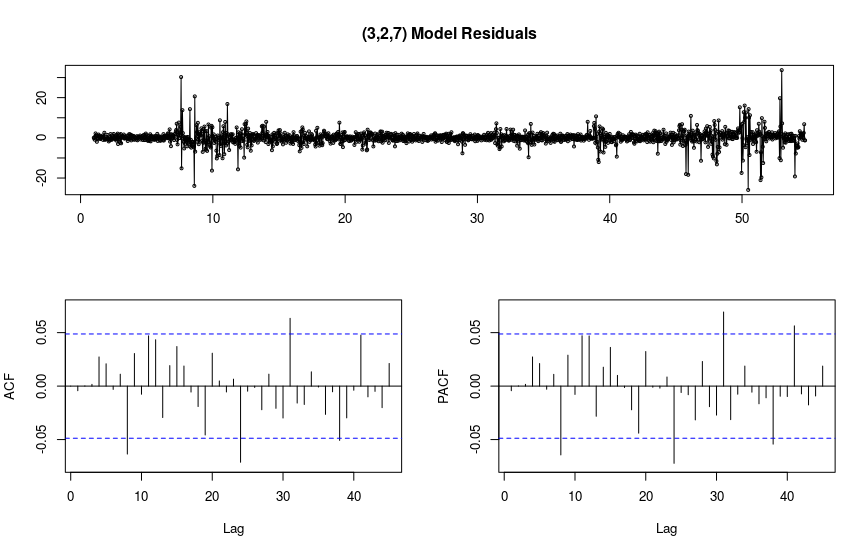
\includegraphics[scale=0.25]{images/ts_images/ARIMAWith327.png}
	\caption{ARIMA with 3,2,7}
	\label{fig: ARIMA with (3,2,7)}
\end{figure}

\subsection{Forecasting}

After generating the above model, we did the forecasting for next 25 elements.

Figure 15 shows the 

\begin{figure}[ht]
	\centering
	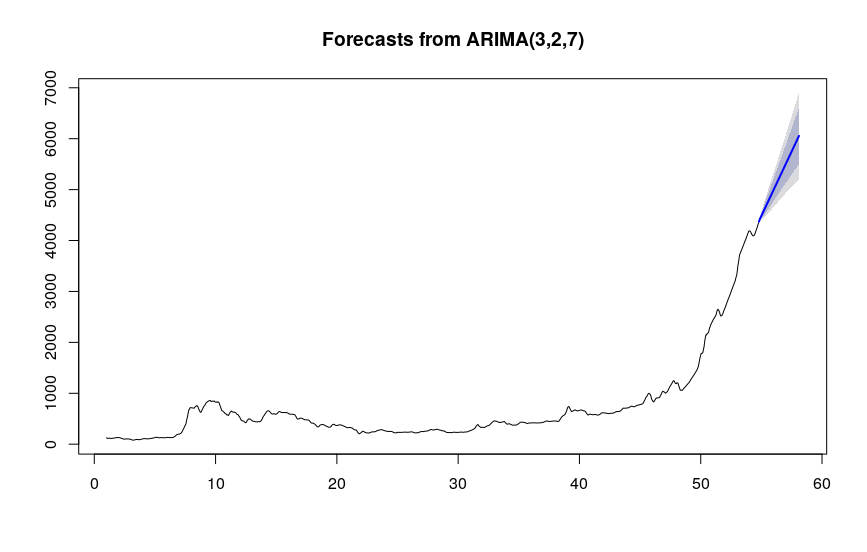
\includegraphics[scale=0.25]{images/ts_images/ForecastWith327.png}
	\caption{ARIMA with 3,2,7}
	\label{fig: Forecast with ARIMA(3,2,7)}
\end{figure}

To confirm the model, we did the forecast for a part of existing data and see how it compares with original data as shown in Figure 16.

\begin{figure}[ht]
	\centering
	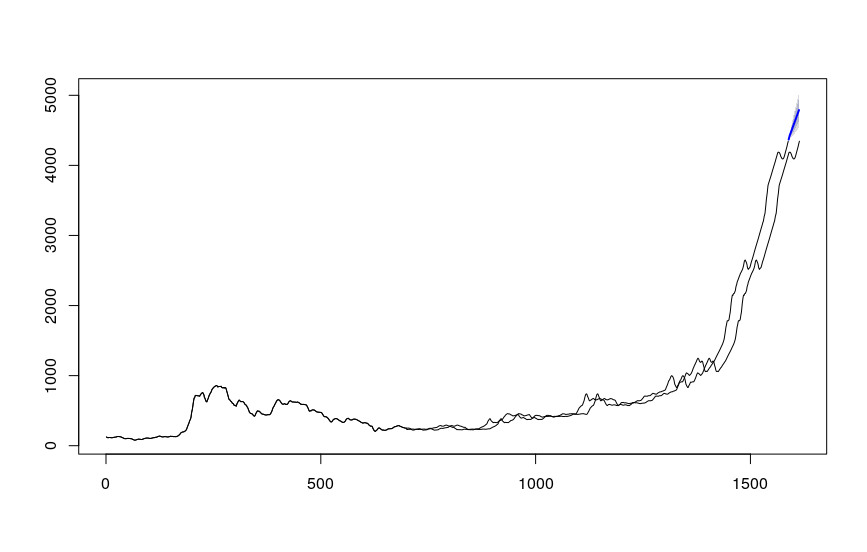
\includegraphics[scale=0.25]{images/ts_images/ForecastedImageH25.png}
	\caption{Forecast and comparision with original data}
	\label{fig: Forecast and Comparision with original data}
\end{figure}

Last we tried future trend prediction which we see matches with our original trend as shown in Figure 17.

\begin{figure}[ht]
	\centering
	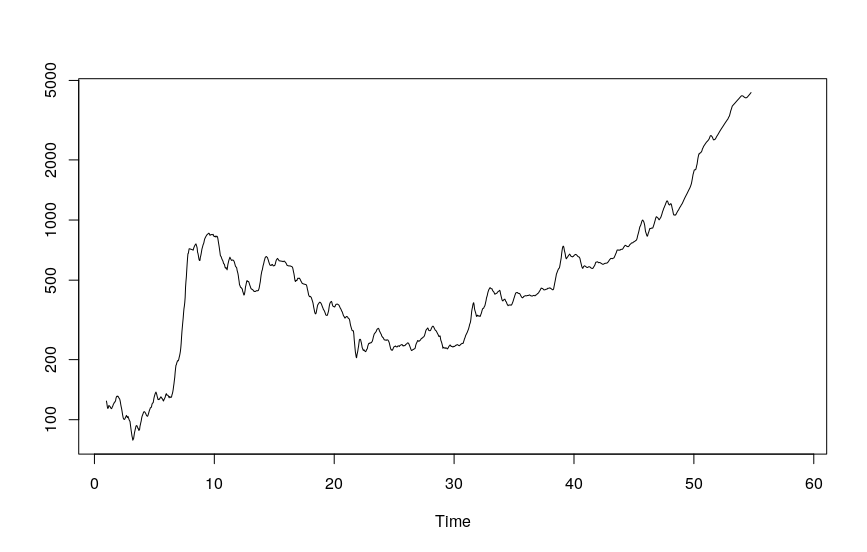
\includegraphics[scale=0.25]{images/ts_images/FutureTrendPrediction.png}
	\caption{Future Trend Prediction}
	\label{fig: Future Trend Prediction}
\end{figure}

\begin{thebibliography}{widestlabel}
	
	\bibitem{1}
	STOCK MARKET TRENDS USING CLUSTER ANALYSIS AND ARIMA MODEL by Joyti Badge, Published in stock Market Trends
	Asian-African Journal using of Economics Cluster Analysis
	and Econometrics, and ARIMA Model Vol. 13, No. 2, 2013: 303-308
	
	\bibitem{2}
	ANALYSIS OF NIFTY FIFTY STOCKS BASED ON K-MEANS CLUSTERING TECHNIQUE FOR STOCK MARKET PREDICTION Dr. T.Chitra kalarani* and S.Indrakala**
	
	\bibitem{3}
	Book named "Data Mining Concepts and Techniques", Jiawei Han, Micheline Kamber, Jian Pei
	
	\bibitem{4}
	https://www.datascience.com/blog/introduction-to-forecasting-with-arima-in-r-learn-data-science-tutorials
	
	\bibitem{5}
	https://www.analyticsvidhya.com/blog/2015/12/complete-tutorial-time-series-modeling/
	
	\bibitem{6}
	https://www.slideshare.net/21\_venkat/arima-26196965
	
	\bibitem{7}
	https://people.duke.edu/~rnau/411arim3.htm
	
\end{thebibliography}

\end{document}